\chapter{Category Inference}
\label{chapter:categories}

To enable semantic filtering and genre-aware recommendations, each book was assigned one or more thematic categories. This process combined zero-shot classification, keyword-based fallback strategies, and confidence-based filtering.

\section{Zero-Shot Classification with BART-MNLI}
Each book's metadata was combined into an \texttt{augmented\_description}, containing title, author, publication year, and description. 
This composite text was passed into the \texttt{facebook/bart-large-mnli} model using Hugging Face’s zero-shot classification pipeline \parencite{bart-large-mnli}.

Thirteen candidate labels were defined (e.g., \textit{Fantasy}, \textit{Love}, \textit{Non-fiction}). For each label, a confidence score was returned. Only scores $\geq 0.4$ were retained to ensure relevance. Books often received multiple labels.

\section{Keyword-Based Fallback Enrichment}
For books with weak model predictions or no confident labels, a curated list of keywords was used to infer likely genres. These fallback rules were only triggered if the corresponding category was not already predicted.

For example:
\begin{itemize}
    \item \textbf{Fantasy:} \textit{wizard}, \textit{magic}, \textit{dragon}
    \item \textbf{Science Fiction:} \textit{cyborg}, \textit{space travel}, \textit{AI}
    \item \textbf{Love:} \textit{romance}, \textit{relationship}, \textit{passion}
\end{itemize}

Fallback tagging increased recall and thematic coverage. Out of 6,572 entries, 4,665 received at least one fallback label.

\section{Refinement and Category Merging}
To reduce noise and improve label interpretability, overlapping or ambiguous categories were merged:
\begin{itemize}
    \item \textit{Biography} + \textit{History} $\rightarrow$ \textit{Historical}
    \item \textit{Suspense} + \textit{Detective} $\rightarrow$ \textit{Mystery}
    \item \textit{Poetry} + \textit{Philosophy} $\rightarrow$ \textit{Philosophy \& Poetry}
\end{itemize}

\begin{figure}[H]
    \centering
    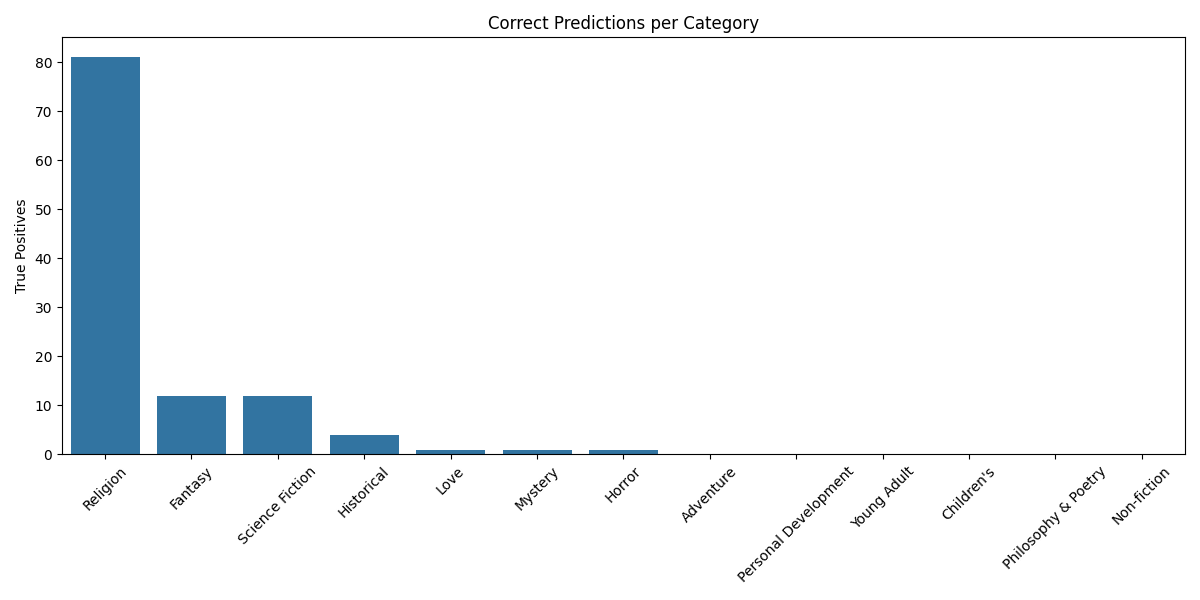
\includegraphics[width=0.9\textwidth]{figures/refine_category_prediction_matches.png}
    \caption{Prediction Matches per Category: Bar chart of true positives per category. Reflects model strength in domains like Fantasy and Love and highlights where fallback logic is critical.}
    \label{fig:refine_category_prediction_matches}
\end{figure}

Per-category precision, recall, and F1 scores were calculated by comparing predicted labels to a cleaned set of original tags. Figure~\ref{fig:refine_category_prediction_matches} shows prediction matches by category.

\section{Confidence Metrics and Filtering}
To prepare the dataset for embedding and indexing, multiple metrics were computed:
\begin{itemize}
    \item \texttt{max\_score} — Highest score among all predicted labels
    \item \texttt{filtered\_avg\_score} — Mean score of predictions $\geq 0.2$
    \item \texttt{score\_std} — Standard deviation across all label scores
    \item \texttt{num\_categories} — Count of confident labels retained
\end{itemize}

A row was retained if it met all of the following:
\begin{itemize}
    \item \texttt{description\_length} $\geq 200$ characters
    \item \texttt{filtered\_avg\_score} $\geq 0.2$
    \item \texttt{max\_score} $\geq 0.4$
    \item \texttt{num\_categories} $> 0$
\end{itemize}

This reduced the dataset from 6,572 to 5,160 high-confidence books.

\section{Length vs Confidence Correlation}
To verify that longer descriptions produce better classifications, correlation coefficients were computed:
\begin{itemize}
    \item Pearson $r = 0.398$, $p < 0.0001$
    \item Spearman $\rho = 0.261$, $p < 0.0001$
\end{itemize}

\begin{figure}[H]
    \centering
    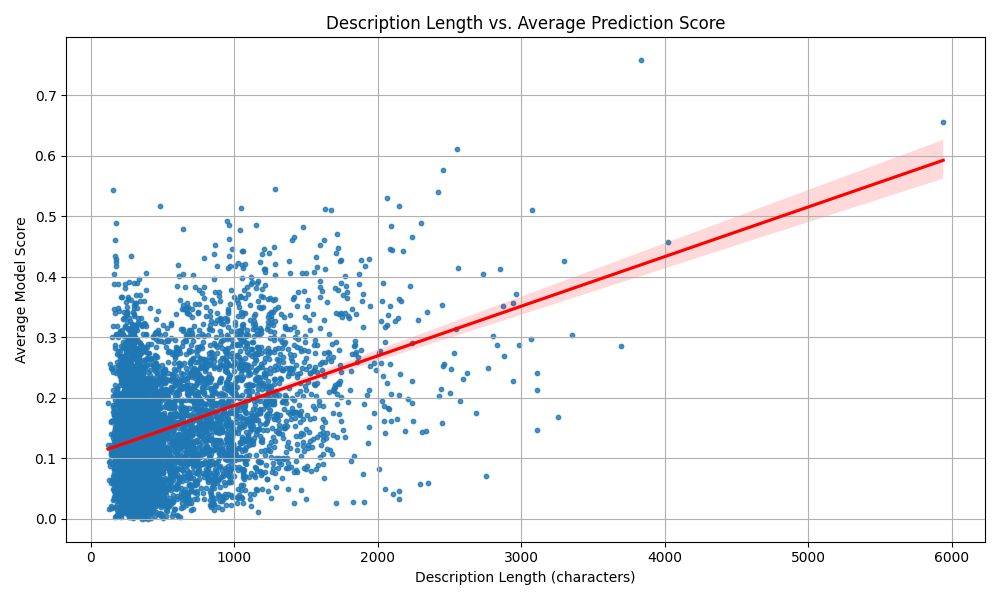
\includegraphics[width=0.9\textwidth]{figures/category_refined_description_length_vs_avg_score.png}
    \caption{Description Length vs. Confidence Score: A regression plot showing the positive correlation between description length and average model confidence.}
    \label{fig:category_refined_description_length_vs_avg_score}
\end{figure}

\begin{figure}[H]
    \centering
    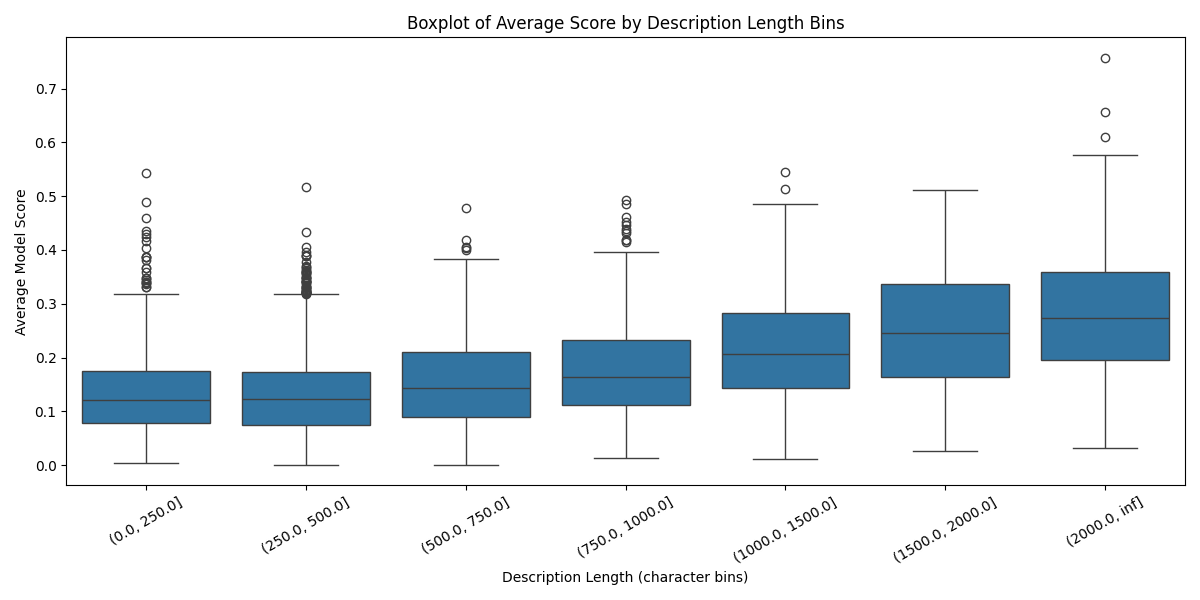
\includegraphics[width=0.9\textwidth]{figures/category_refined_avg_score_by_length_bin.png}
    \caption{Score by Length Bin: A boxplot displaying score variation across binned description lengths.}
    \label{fig:category_refined_avg_score_by_length_bin}
\end{figure}

These results indicate a moderate positive relationship. Figure~\ref{fig:category_refined_description_length_vs_avg_score} visualizes the regression, while Figure~\ref{fig:category_refined_avg_score_by_length_bin} shows variation across bins.

These findings supported a minimum \texttt{description\_length} of 200 characters during filtering.